%%%
 %
 % Copyright (C) 2020 Ángel Iván Gladín García
 %
 % This program is free software: you can redistribute it and/or modify
 % it under the terms of the GNU General Public License as published by
 % the Free Software Foundation, either version 3 of the License, or
 % (at your option) any later version.
 %
 % This program is distributed in the hope that it will be useful,
 % but WITHOUT ANY WARRANTY; without even the implied warranty of
 % MERCHANTABILITY or FITNESS FOR A PARTICULAR PURPOSE.  See the
 % GNU General Public License for more details.
 %
 % You should have received a copy of the GNU General Public License
 % along with this program.  If not, see <http://www.gnu.org/licenses/>.
%%%

%%%%%%%%%%%%%%%%%%%%%%%%%%%%%%%%%%%%%%%%%%%%%%%%%%%%%%%%%%%%%%%%%%%%%%%%%%%%%%%%%%%%%%%%%
\documentclass[12pt,letterpaper]{article}
\usepackage[margin=.65in]{geometry}
\usepackage[utf8]{inputenc}
\usepackage[spanish]{babel}
\decimalpoint

\usepackage{listings}
\usepackage{color}
\usepackage{graphicx}
\usepackage{enumerate}
\usepackage{enumitem}
\usepackage{float}

\usepackage{longtable}
\usepackage{hyperref}
\usepackage{commath}

\usepackage{bbm}
\usepackage{dsfont}
\usepackage{mathrsfs}
\usepackage{amsmath,amsthm,amssymb}
\usepackage{mathtools}
\usepackage{longtable}

\usepackage{tikz}
\usetikzlibrary{trees}
\usepackage{verbatim}

%%%%%%%%%%%%%%%%%%%%%%%%%%%%%%%%%%%%%%%%%%%%%%%%%%%%%%%%%%%%%%%%%%%%%%%%%%%%%%%%%%%%%%%%%%%%%%%%5

\usepackage{import}

\usepackage[utf8]{inputenc}

\usepackage{listings}
\usepackage{color}
%%%%%%%%%%%%%%%%%%%%%%%%%%%%%%%%%%%%%%%%%%%%%%%%%%%%%%%%%%%%%%%%%%%%%%%%%%%%%%%%%%%%%%%%%


%%%%%%%%%%%%%%%%%%%%%%%%%%%%%%%%%%%%%%%%%%%%%%%%%%%%%%%%%%%%%%%%%%%%%%%%%%%%%%%%%%%%%%%%%
\newcommand{\Z}{\mathbb{Z}}
\newcommand{\N}{\mathbb{N}}
\newcommand{\Q}{\mathbb{Q}}
\newcommand{\R}{\mathbb{R}}
\newcommand{\Pro}{\mathds{P}}
\newcommand{\Oh}{\mathcal{O}} %% Notacion "O"
\newcommand{\lra}{\longrightarrow}
\newcommand{\ra}{\rightarrow}
\newcommand{\ord}{\text{ord}}
\newcommand{\sol}{\textbf{\underline{Solución}: }} %% Solucion
\newcommand{\af}{\textbf{\underline{Afirmación}: }}
\newcommand{\cej}{\textbf{\underline{Contraejemplo}: }}

%%%%%%%%%%%%%%%%%%%%%%%%%%%%%%%%%%%%%%%%%%%%%%%%%%%%%%%%%%%%%%%%%%%%%%%%%%%%%%%%%%%%%%%%%

\begin{document}

%%%%%%%%%%%%%%%%%%%%%%%%%%%%%%%%%%%%%%%%%%%%%%%%%%%%%%%%%%%%%%%%%%%%%%%%%%%%%%%%%%%%%%%%%
\title{
        Universidad Nacional Autónoma de México\\
        Facultad de Ciencias\\
        Teoría de los Números II\\
    \vspace{.5cm}
    \large
        \textbf{Tarea 1}
}
\author{
    Ángel Iván Gladín García\\
    No. cuenta: 313112470\\
    \texttt{angelgladin@ciencias.unam.mx}
}
\date{23 de Marzo 2020}
\maketitle
%%%%%%%%%%%%%%%%%%%%%%%%%%%%%%%%%%%%%%%%%%%%%%%%%%%%%%%%%%%%%%%%%%%%%%%%%%%%%%%%%%%%%%%%%

%%%%%%%%%%%%%%%%%%%%%%%%%%%%%%%%%%%%%%%%%%%%%%%%%%%%%%%%%%%%%%%%%%%%%%%%%%%%%%%%%%%%%%%%%
\newtheorem{theorem}{Teorema}
\newtheorem{example}{Ejemplo}
\newtheorem{corollary}{Corolario}
\newtheorem{lemma}{Lemma}
\newtheorem{definition}{Definicion}
\newtheorem{prop}{Proposicion}
%%%%%%%%%%%%%%%%%%%%%%%%%%%%%%%%%%%%%%%%%%%%%%%%%%%%%%%%%%%%%%%%%%%%%%%%%%%%%%%%%%%%%%%%%

%%%%%%%%%%%%%%%%%%%%%%%%%%%%%%%%%%%%%%%%%%%%%%%%%%%%%%%%%%%%%%%%%%%%%%%%%%%%%%%%%%%%%%%%%
\subsection*{Prueba del Teorema de los números pentagonales de Euler}

En clase vimos que los númeors pentagonales se pueden ver como,

\begin{figure}[H]
    \centering
    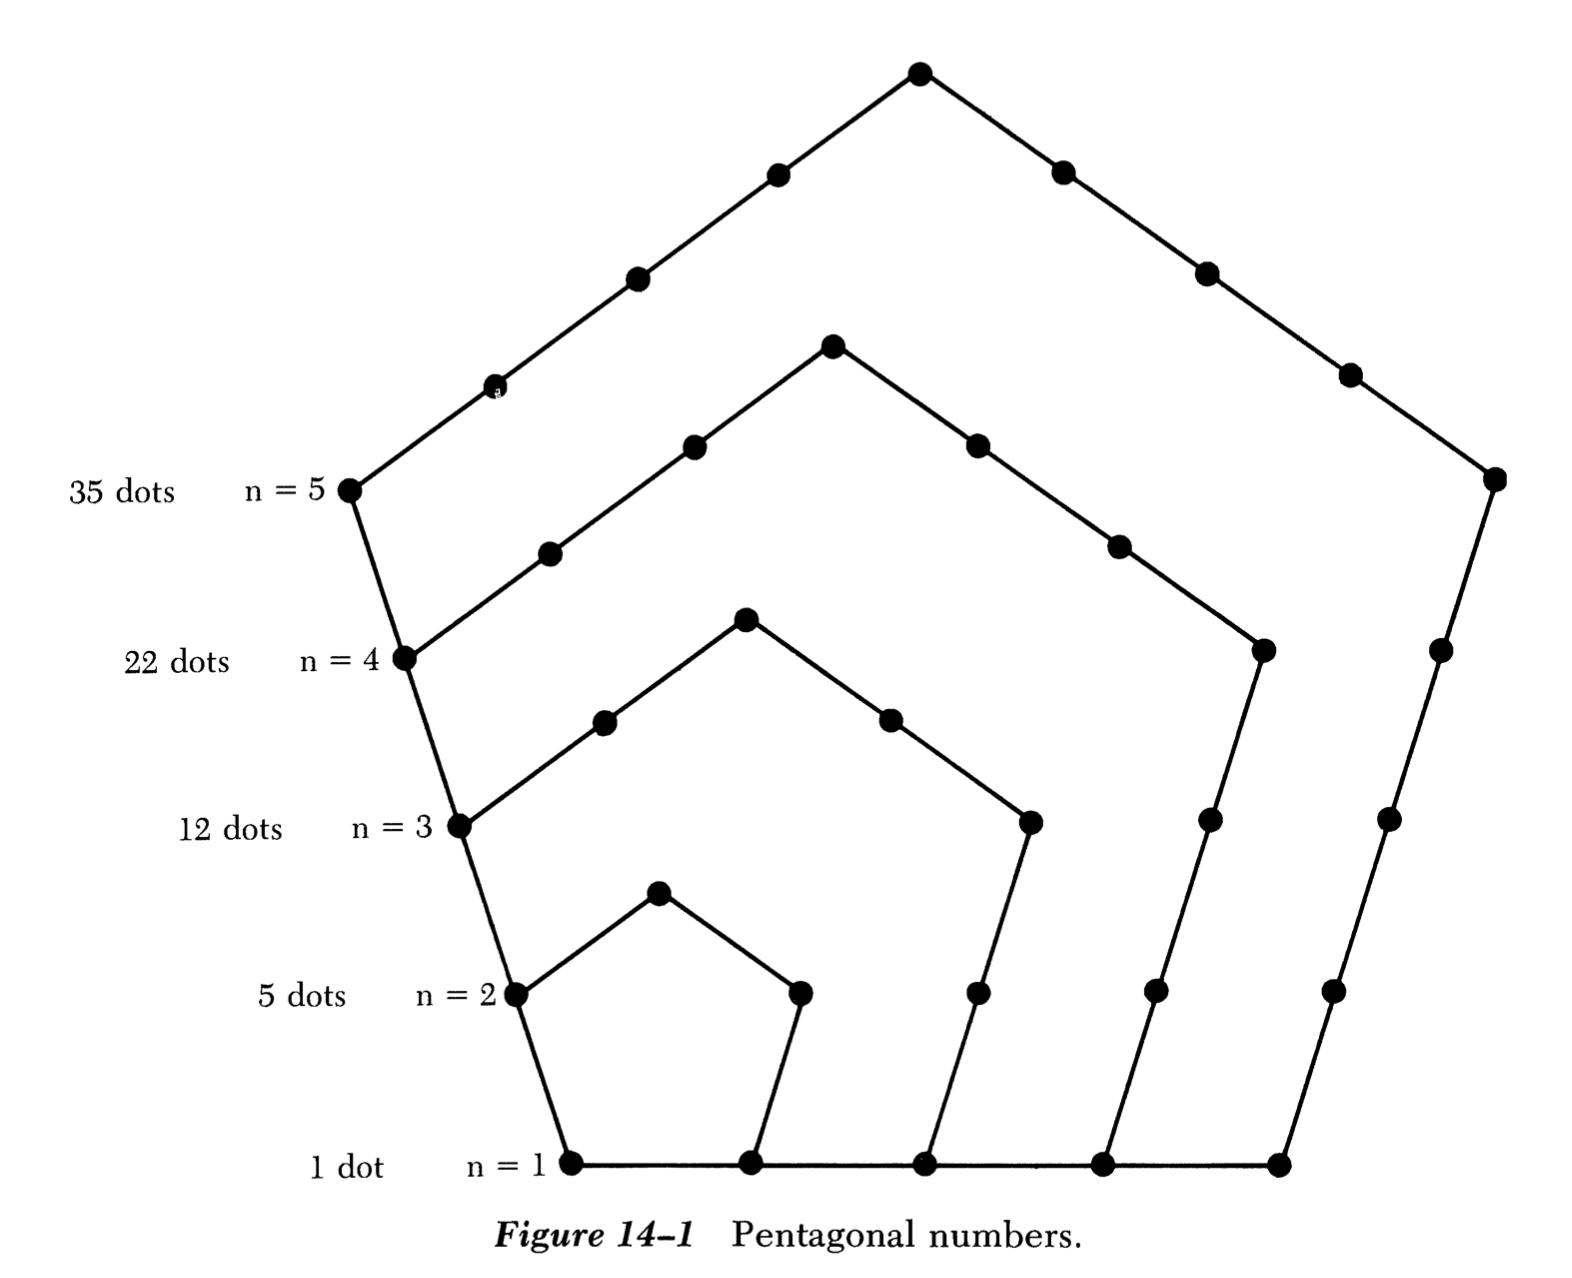
\includegraphics[scale=0.3]{assests/1.png}
    \caption{Vemos que el número de los puntos adentro y en el $n$-ésimo pentágono es
    $\frac{n(3n-1)}{2}$. Por lo que los números $1,5,12,\ldots,\frac{n(3n-1)}{2},\ldots$ son
    llamados números pentagonales.}
\end{figure}

Usando el \textit{Producto Triple de Jabobi} que enuncia lo siguiente:
\begin{theorem}
    Si $z \not= 0$ y $|q| < 1$, entonces,
    \[ \prod_{n=0}^{\infty} (1-q^{2n+2})(1 +zq^{2n+1})(1+z^{-1}q^{2n+1}) =
        \sum_{n=-\infty}^{\infty} q^{n^2}z^n\]
\end{theorem}

\begin{theorem}[Números pentagonales]
\[ \sum_{n=-\infty}^{\infty} (-1)^{n} q^{n\frac{3n-1}{2}} =
    \prod_{n=1}^{\infty} (1-q^n) \text{ donde $|q|<1$.} \]
\begin{proof}
Sustituyendo $q$ por $q^{\frac{3}{2}}$ y $z$ por $-\sqrt{q}$ en lo siguiente:

\begin{align*}
    &\prod_{n=1}^{\infty} (1-q^{2n})(1+q^{2n-1}z^2) \left(1+\frac{q^{2n-1}}{z^2} \right)\\
        &= \prod_{n=1}^{\infty} (1 + q^{\frac{3(2n-1)}{2}}(-\sqrt{q}))
            \left(1+\frac{q^{\frac{3(2n-1)}{2}}}{-\sqrt{q}} \right) (1-q^{3n})\\
        &= \prod_{n=1}^{\infty}(1-q^{\frac{6n-3+1}{2}})
            (1-q^{\frac{6n-3+1}{2}})(1-q^{3n})\\
        &= \prod_{n=1}^{\infty}(1-q^{3n-1})(1-q^{3n-2})(1-q^{3n})\\
        &= \prod_{n=1}^{\infty}(1-q^n)
\end{align*}

Por la misma sustitución,

\begin{align*}
    \sum_{n=\infty}^{\infty} q^{n^2}z^{2n}
        &= \sum_{n=\infty}^{\infty} q^{\frac{3n^2}{2}} (-\sqrt{q})^n\\
        &= \sum_{n=\infty}^{\infty} (-1)^n q^{\frac{3n^2 + n}{2}}\\
        &= \sum_{n=\infty}^{\infty} (-1)^n q^{\frac{(3n - 1)n}{2}}\\
\end{align*}

Donde la última igualdad es obtenida invirtiendo el índice de la suma y factorizando el exponente. Por el
Producto Triple de Jabobi son iguales.
\end{proof}

\end{theorem}

%%%%%%%%%%%%%%%%%%%%%%%%%%%%%%%%%%%%%%%%%%%%%%%%%%%%%%%%%%%%%%%%%%%%%%%%%%%%%%%%%%%%%%%%%


%%%%%%%%%%%%%%%%%%%%%%%%%%%%%%%%%%%%%%%%%%%%%%%%%%%%%%%%%%%%%%%%%%%%%%%%%%%%%%%%%%%%%%%%%

%% ANDREWS, George. 1971. Number Theory. EUA: Saunders Company.

%%%%%%%%%%%%%%%%%%%%%%%%%%%%%%%%%%%%%%%%%%%%%%%%%%%%%%%%%%%%%%%%%%%%%%%%%%%%%%%%%%%%%%%%%

\end{document}
